\section{Experimental Evaluation}
\subsection{Experimental Setup}
For our experiments, we used a cluster with 12 nodes running Linux O.S. (kernel 3.10) and Apache Spark 2.4. Each node has 8 cores (i.e. 96 cores in total), each core with an Intel Xeon CPU at 1.70GHz and 4GB of main memory.
To evaluate the various approaches, we used 3 synthetic datasets, with different characteristics as described in table \ref{tab:datasets}. To create these datasets we used the SUMO simulator \cite{SUMO2012} and imported the traffic networks of Berlin and Los Angeles from OpenStreetMap \cite{haklay2008openstreetmap}. We used the SUMO setting for pedestrians, and created 10K, 25K and 50K pedestrian trajectories. We set the total duration to 10, 30 and 60 min respectively. The generator reported the positions of these moving pedestrians every minute.

\begin{table}
    \centering
    \begin{tabular}{cccc}
        \hline
        Dataset & Number of Trajectories & Total number of points & Maximum Duration (min) \\
        \hline
         Berlin10K &  10000 & 97526 & 10\\ 
         LA25K &  25000 & 1495637 & 30\\
         LA50K &  50000 & 2993517 & 60\\
         \hline
    \end{tabular}
    \caption{Datasets}
    \label{tab:datasets}
\end{table}

For the partitioning phase we used a quadtree structure (other indices can be used as well; the advantage of the quadtree is that it tries to create nodes with similar number of objects). 
Our input is a set of points \textit{(traj-id, x,y,t)}. To build the quadtree, we sample 1\% of the input and insert this subset of points to an empty quadtree. For a quadtree, the user needs to set a parameter for the node capacity $c$. When the number of points that fall in a node overpass $c$ the node splits. After all sample points are inserted, we use the Minimum Bounding Rectangles (MBRs) of the leaves as the partitions of our approach. All the remaining points are then inserted in these fixed partitions (i.e., no more splitting occurs). Each partition will be assigned to a different cluster node which will run a sequential version of BFE or PSI, run locally on the points of that partition.

\subsection{Optimal number of partitions for phase 1.}
Clearly the capacity parameter $c$ directly affects the number of partitions. A low value of $c$ leads to a large number of partitions. This in return will generate many smaller jobs to be distributed over the cluster. However, the cost of transmission and possibly replication increases, which could become a bottleneck.  On the other hand, large $c$ implies a smaller number of partitions, which will create larger individual jobs, increasing the time response required by the sequential algorithm in each partition. 

Figure \ref{fig:optimal_performance} shows the execution time (in seconds) for finding the maximal disks (phase 1) for a given time instant, under different values of $c$ and for various values of $\varepsilon$. The LA25K dataset was used for these experiments. 
Consider the case $\varepsilon = 20m$; clearly there is a value of $c$ that minimizes the time to find the maximal disks ($c=100$, which corresponds to around 1300 partitions). 
It can also be seen that the optimal value for $c$ varies depending on $\varepsilon$.  For example, for smaller $\varepsilon = 2m$, the execution time is minimized for a larger capacity  $c=500$ (which corresponds to around 250 partitions).
When $\varepsilon$ is large, there will be larger number of pairs and thus maximal disks to compute. Using a smaller $c$ creates more partitions (for the same spatial area) thus reducing the amount of work per partition.

\begin{figure}
    \centering
    \begin{tabular}{c c}
         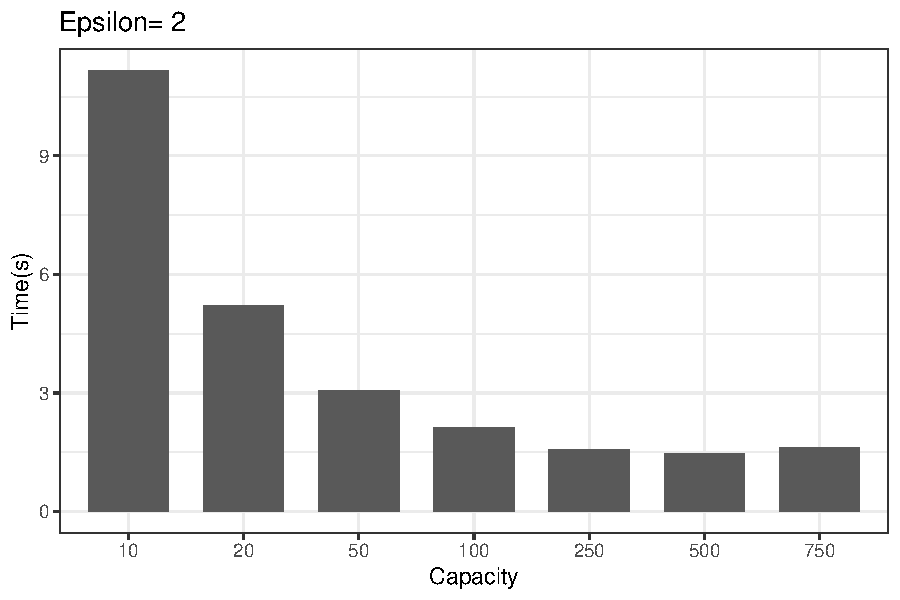
\includegraphics[width=0.45\linewidth]{figures/plots/01_optimal_performance/pflockE2_by_capacity.pdf} & 
         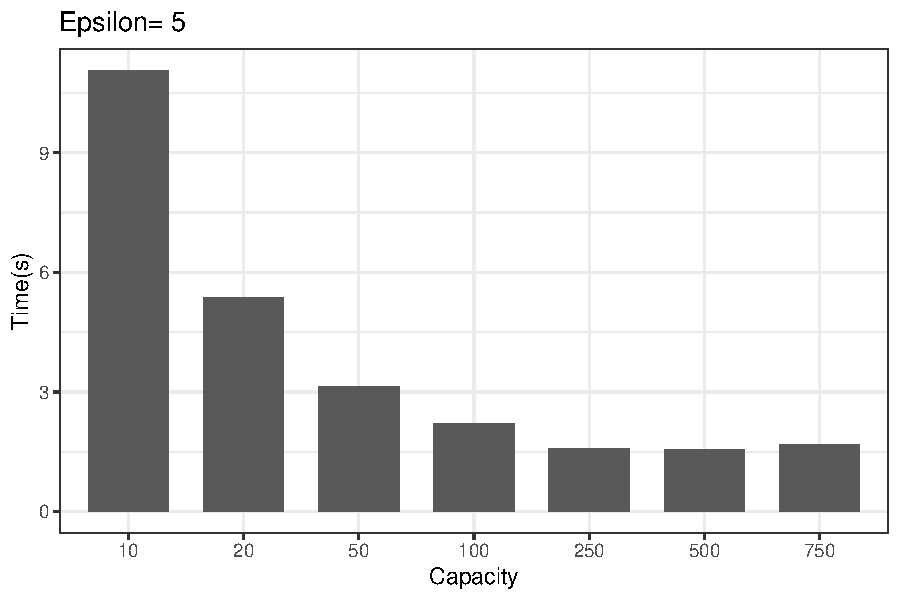
\includegraphics[width=0.45\linewidth]{figures/plots/01_optimal_performance/pflockE5_by_capacity.pdf} \\
         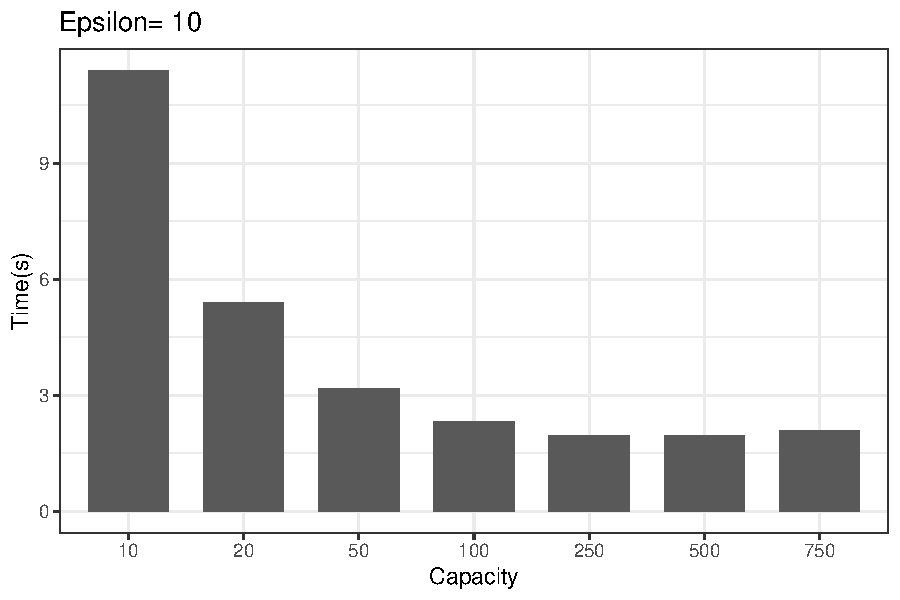
\includegraphics[width=0.45\linewidth]{figures/plots/01_optimal_performance/pflockE10_by_capacity.pdf} &
         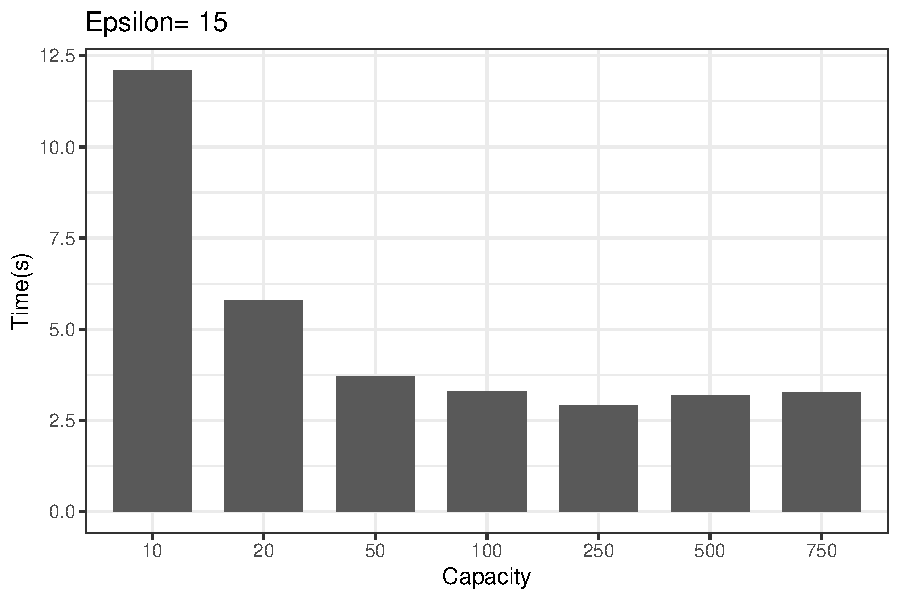
\includegraphics[width=0.45\linewidth]{figures/plots/01_optimal_performance/pflockE15_by_capacity.pdf} \\ 
         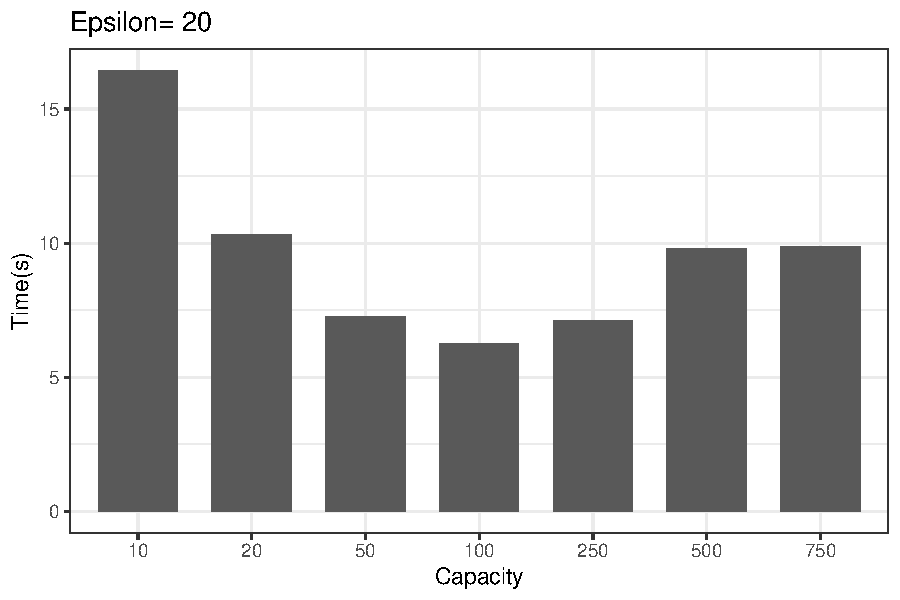
\includegraphics[width=0.45\linewidth]{figures/plots/01_optimal_performance/pflockE20_by_capacity.pdf} & \\
    \end{tabular}
    \caption{Execution time testing different values for Capacity ($c$) and Epsilon  $\varepsilon$).}\label{fig:optimal_performance}
\end{figure}

Having set the optimal value of $c$ for a given $\varepsilon$ value, we further explored the behavior of BFE and PSI for the most `demanding' partitions, that is, those partitions that took the most time to compute phase 1. Since partitions run in parallel on different cores, these are the partitions that will affect the overall performance.  

\subsection{Analyzing most costly partitions.}
We first identified the top-10 partitions that take most time to run the BFE algorithm with $\varepsilon$ = 20 meters. For these specific partitions we run both BFE and PSI while varying $\varepsilon$ from 10 to 20 meters. Figure \ref{fig:top_time_partitions} 
shows the phase 1 execution times; we see that the PSI performance was consistently better than BFE. 

\begin{figure}
    \centering
    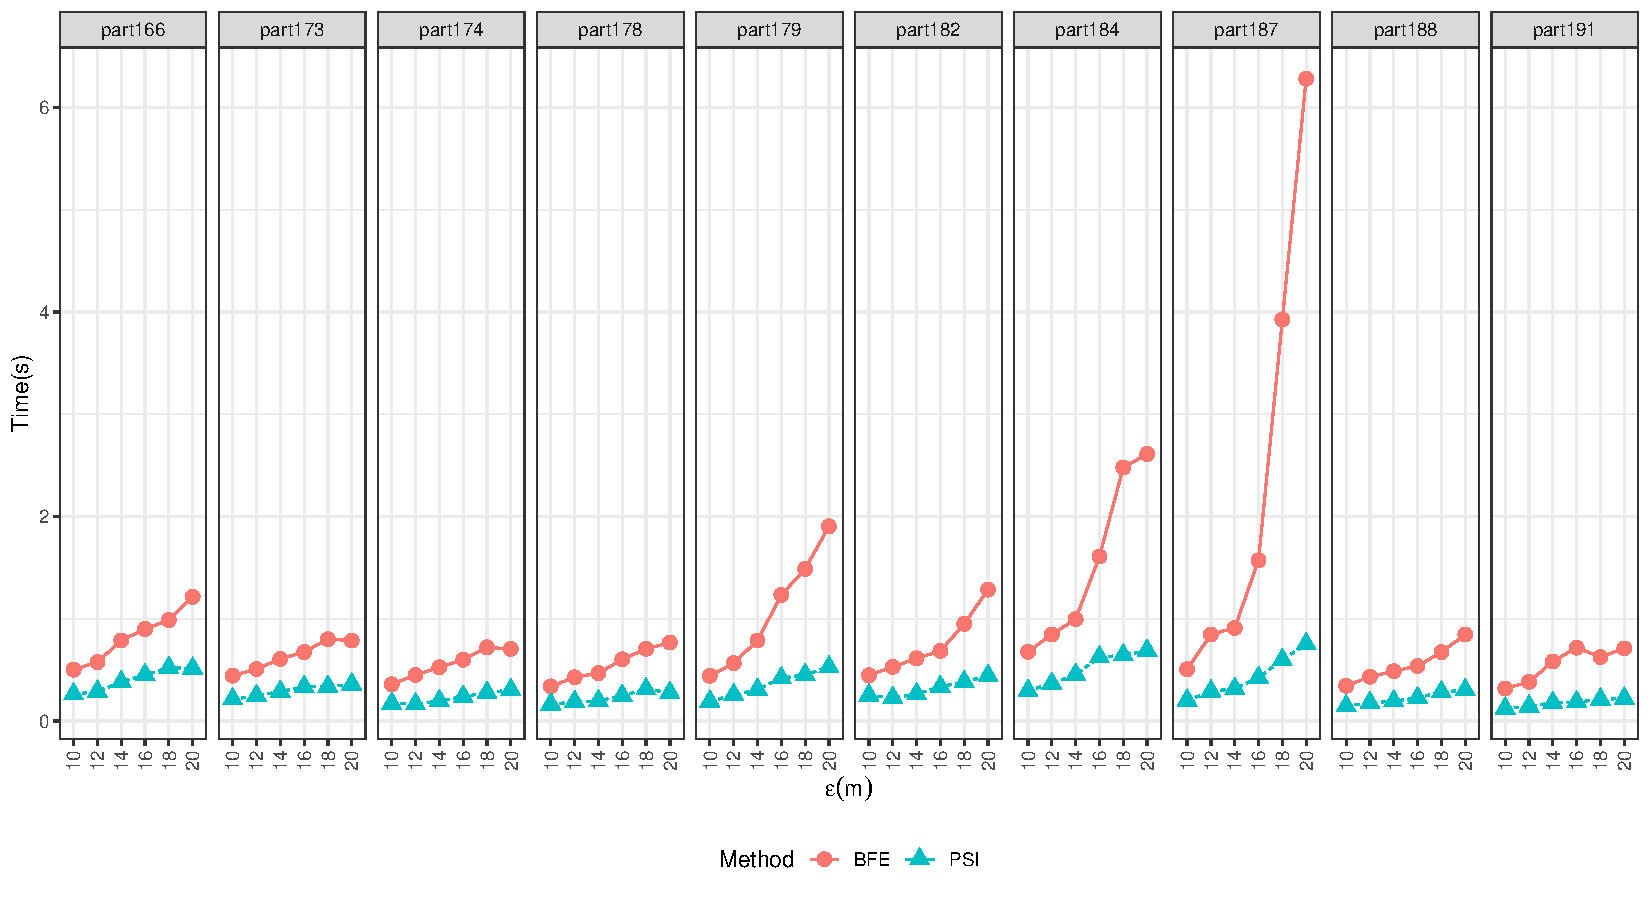
\includegraphics[width=\linewidth]{figures/plots/03_top_time_partitions/top_time_partitions.pdf}
    \caption{Comparing the performance of PSI and BFE for time consuming  partitions.}\label{fig:top_time_partitions}
\end{figure}

We further examined what causes some partitions to take more time than others. Figure \ref{fig:pairs_performance} shows the phase 1 execution times per partition while varying $\varepsilon$ from 10m to 20m. Partitions are ordered by the number of pairs they contain. A first observation is that we $\varepsilon$  increases, the number of pairs also increase since higher $\varepsilon$  allows for more maximal disks. For example, for $\varepsilon$=10m the highest number of pairs in a partition is around 1800. In contrast, for $\varepsilon$ =20m, there are partitions with almost 4000 pairs. Another observation is that BFE is more affected than PSI by the density of pairs in a partition. This is depicted more clearly for $\varepsilon$ =18m or 20m. As mentioned earlier, the flexible boxes that PSI uses (see Figure \ref{fig:square}) better identify the points needed for computing the pairs; instead BFE uses a fixed grid cell. 

A final observation is that there are few partitions that take much more time than others, those that are more dense with pairs (as this relates to the number of disks that have to be computed and later pruned). For example, the partition that takes more time for $\varepsilon$ =20m in the Figure, is the one with most pairs (which shows as partition 187 in Figure \ref{fig:top_time_partitions}). 

We thus further examine how the processing for phase 1 is divided in the most `demanding' partition. Figure \ref{fig:dense_stages}.a (.b) shows the processing taken by each of the phase 1 stages (see Figure \ref{fig:example}) of BFE (respectively PSI) for partition 187. 
It can be seen that the most expensive stage is the final procedure of filtering the disks whose points are included in other disks, that is identifying the `Maximal' disks (shown as Maximals in the figure). This is because both BFE and PSI need to scan a large set of candidate disks looking for those which could contain others and remove the rest. It is clear that this processing increases as $\varepsilon$ increases, since the number of pairs and subsequent candidates disks also increases with $\varepsilon$.

\begin{figure}
    \centering
    \begin{tabular}{c c}
        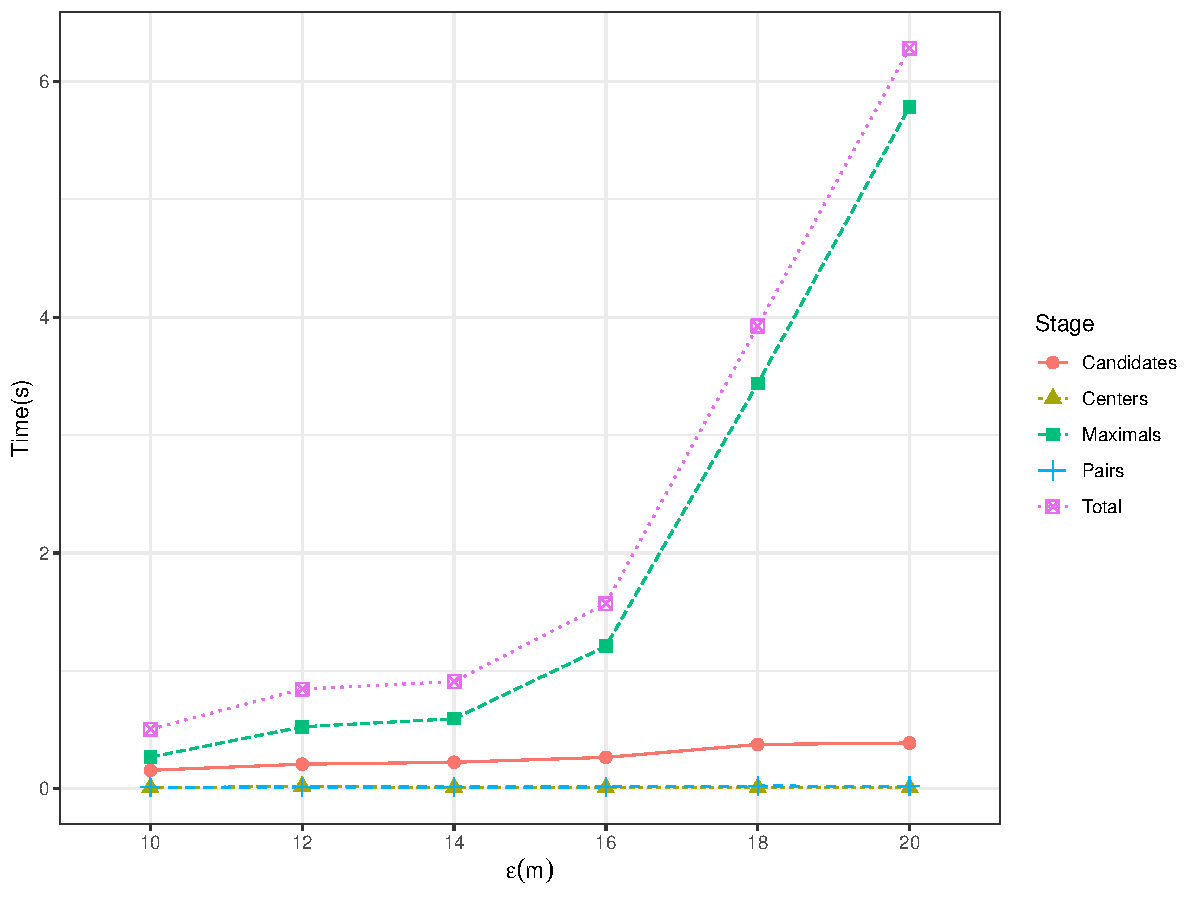
\includegraphics[width=0.49\linewidth] {figures/plots/09_dense_stages/dense_stages_bfe.pdf} &
        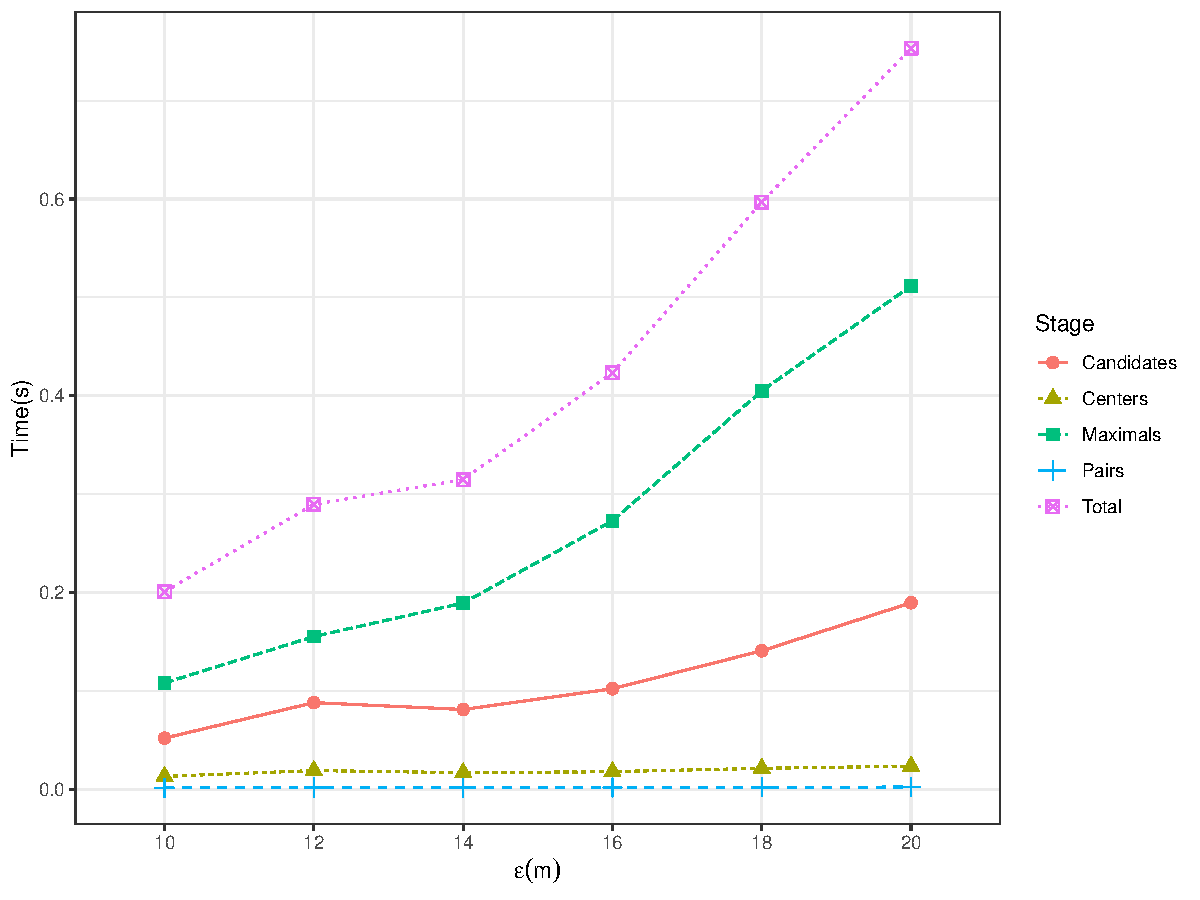
\includegraphics[width=0.49\linewidth] {figures/plots/09_dense_stages/dense_stages_psi.pdf} \\
        (a) & (b) \\
    \end{tabular}
    \caption{Processing time for the stages of Phase 1, in (a) BFE, (b) PSI.}\label{fig:dense_stages}
\end{figure}

\begin{figure}
    \centering
    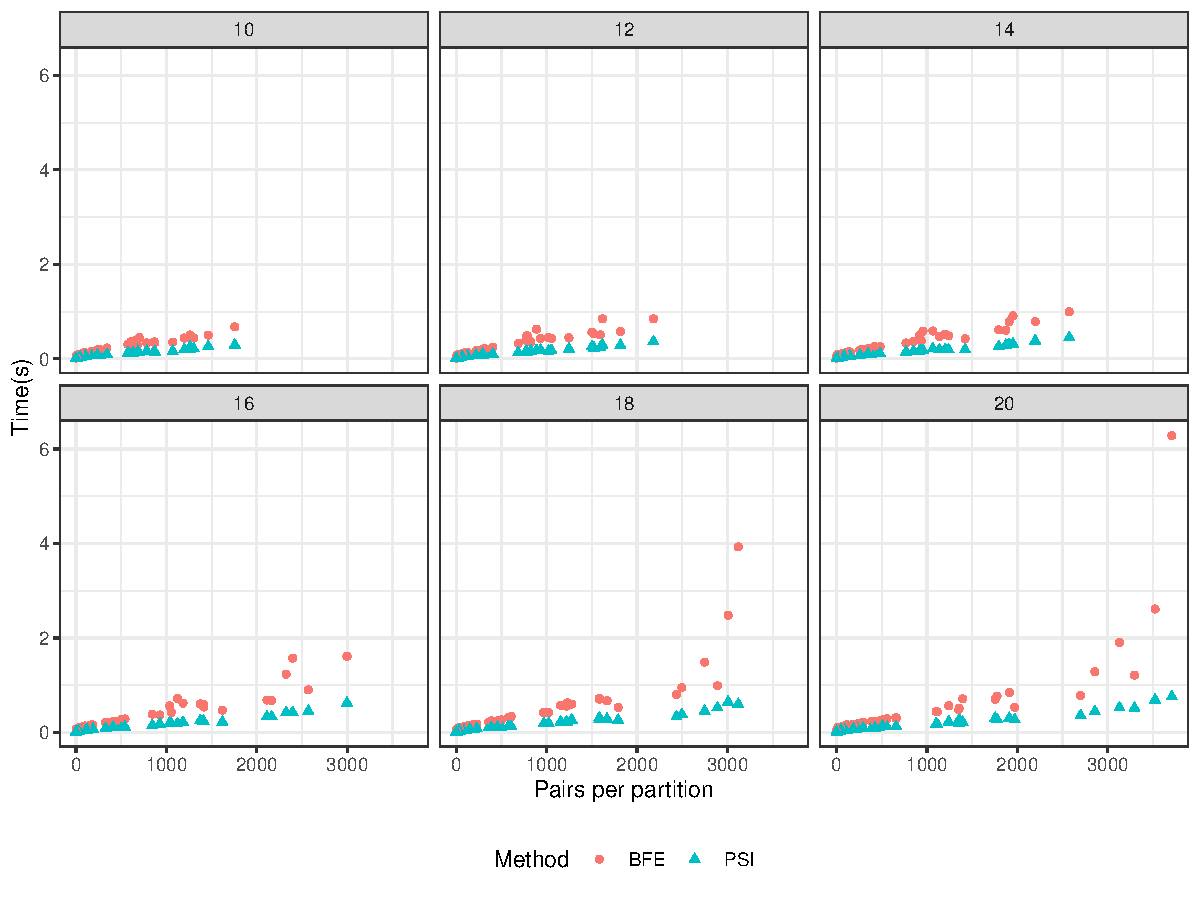
\includegraphics[width=0.85\linewidth]{figures/plots/04_pairs_performance/pairs_performance.pdf}
    \caption{Execution time for pairs/disks finding in the dense partition.}\label{fig:pairs_performance}
\end{figure}

\subsection{Can we reduce pruning time?}
Dense areas are problematic for pruning as they are very sensitive to an increase in the value of $\varepsilon$, creating an enormous number of pairs. Therefore, we explored ideas that may lead to more effective grouping of points. It should be noted that density based spatial clustering approaches (e.g. DBSCAN \cite{dbscan}) will not work since very dense areas will result in one large cluster, thus not solving the issue. Moreover, clustering does not enforce strong relationship among all elements in the cluster (which is something we need for a flock: all points are within $\varepsilon$ from each other).

Instead, we explored graph-oriented clustering, and in particular the notion of \textit{maximal cliques}. In an undirected graph, a maximal clique is a subset of vertices where each vertex is directly connected to every other vertex in the subset; further the subset is maximal in the sense that it cannot be further extended by adding a new vertex \cite{tomita_clique_2013, bron_algorithm_1973}. 
One could consider the points in a partition as the vertices of an undirected graph and add edges that connect those pairs of points that are within $\varepsilon$ distance. 
Finding the set of maximal cliques in this graph will provide subsets of points which are directly connected to ALL the other members in the subset, that is, all points in the subset are at most $\varepsilon$ apart from each other and no other point could be added to the subset. 
However, not all maximal cliques are maximal disks. 
A maximal clique is a maximal disk if it has at least $\mu$ points and can be enclosed by a disk with radius $\frac{\varepsilon}{2}$.

To check this condition, we introduce the concept of Minimum Bounding Circle (MBC) \cite{welzl_mbc_1991}. Given a set of points in the Euclidean space, a MBC is the smallest circle that contains all the points. For each maximal clique found in a partition, we could quickly check if the points in this clique are all inside a MBC with diameter $\varepsilon$. If this is the case, we can directly report that set of points and their MBC as a maximal disk. However those cliques that not fulfill the restriction must be evaluated in the traditional way (i.e., for the clique points we must compute centers, find disks, prune disks as in Figure \ref{fig:MF_flowchart}).

To evaluate the cliques that do not pass the above condition, we used two variants. The first one (termed COLLECT) collects the points from \textit{all} the cliques that are not reported as maxima disks, removes duplicates (points that appear in many cliques) and apply the traditional method of pruning for the whole set. In the second (noted as EACH) we apply the pruning procedure over the points of each such clique independently. Figure \ref{fig:cmbc_variants} shows the performance of the variants compared with the time employed by BFE for the same stage (a) and the PSI (b).  It turns out that the performance of the variants does not improve the execution time. Looking more closely at each approach we can observe that while finding the cliques (and their MBCs) does not take much time, nor many of these cliques are maximal disks. The overhead to find the maximal disks from the remaining cliques is large, making the original approach faster for both the BFE and PSI.

\begin{figure}
    \centering
    \begin{tabular}{c c}
        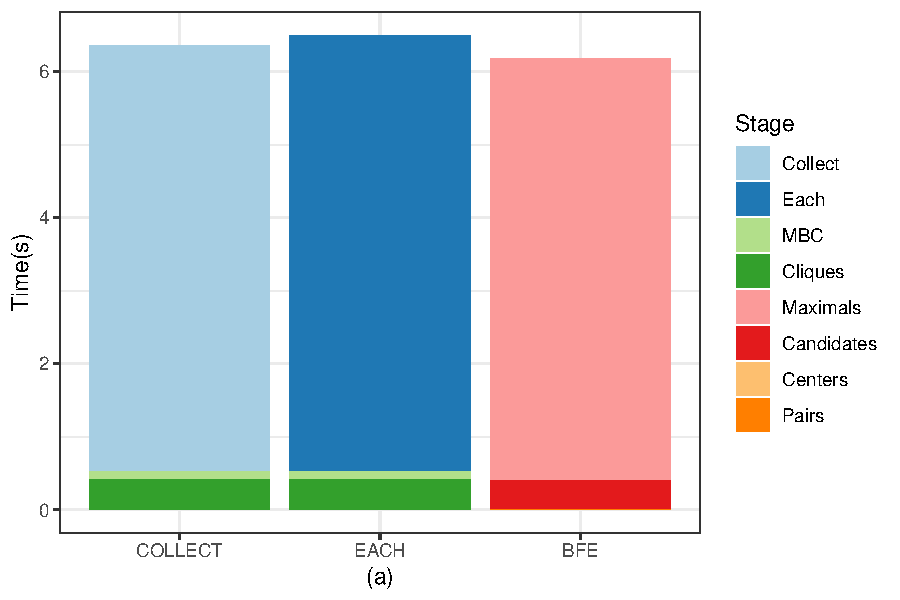
\includegraphics[width=0.49\linewidth] {figures/plots/10_cmbc_variants/cmbc_bfe.pdf} &
        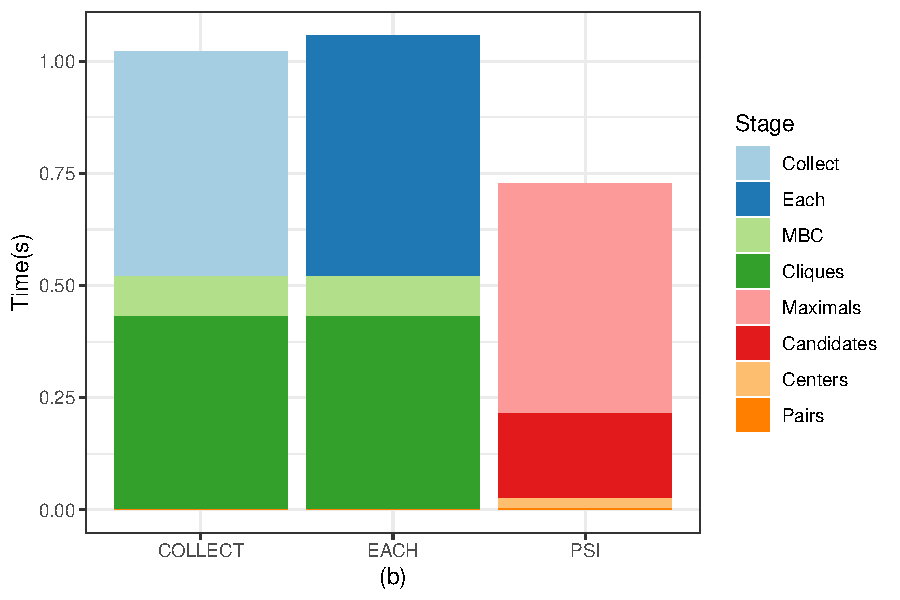
\includegraphics[width=0.49\linewidth] {figures/plots/10_cmbc_variants/cmbc_psi.pdf} \\
        (a) & (b) \\
    \end{tabular}
    \caption{Execution time of the Cliques approach compared to (a) standard BFE and (b) standard PSI.}\label{fig:cmbc_variants}
\end{figure}

\subsection{Uniform dataset.}
To better examine the relative behavior of the scalable BFE and PSI approaches, we also considered a synthetic dataset where we could control the values of $c$, $\varepsilon$ and the point density. We used a fixed square area of 1000m x 1000m and placed 25K, 50K, 75K and 100K points uniformly distributed in this area. 
We used various quadtree capacities ($c$ equal to 100, 200 and 300) that gave us different number of partitions (see Table ~\ref{tab:uniform_ncells}). We run both BFE and PSI for finding the maximal disks of phase 1, using different $\varepsilon$ values (from 1m to 5m). The results appear in Figure \ref{fig:uniform_performance}. While we again see that overall PSI has better performance than BFE, there are cases (for small $\varepsilon$ values) where BFE is better. In those cases, the small $\varepsilon$ creates fewer pairs and the ordering that PSI requires is an overhead. Nevertheless, in the remaining experiments where we consider the temporal joins (phase 2, flock creation) we concentrate on the scalable performance of PSI. 

\begin{table}
    \centering
    \begin{tabular}{c|cccc}
              & 25K & 50K  & 75K  & 100K \\
        \hline
        c=100 & 544 & 1024 & 1024 & 2185 \\
        c=200 & 256 & 514  & 1024 & 1024 \\
        c=300 & 256 & 514  & 481  & 1024 \\
    \end{tabular}
    \caption{Number of partitions by capacity and number of points in uniform datasets.}
    \label{tab:uniform_ncells}
\end{table}

\begin{figure}
    \centering
    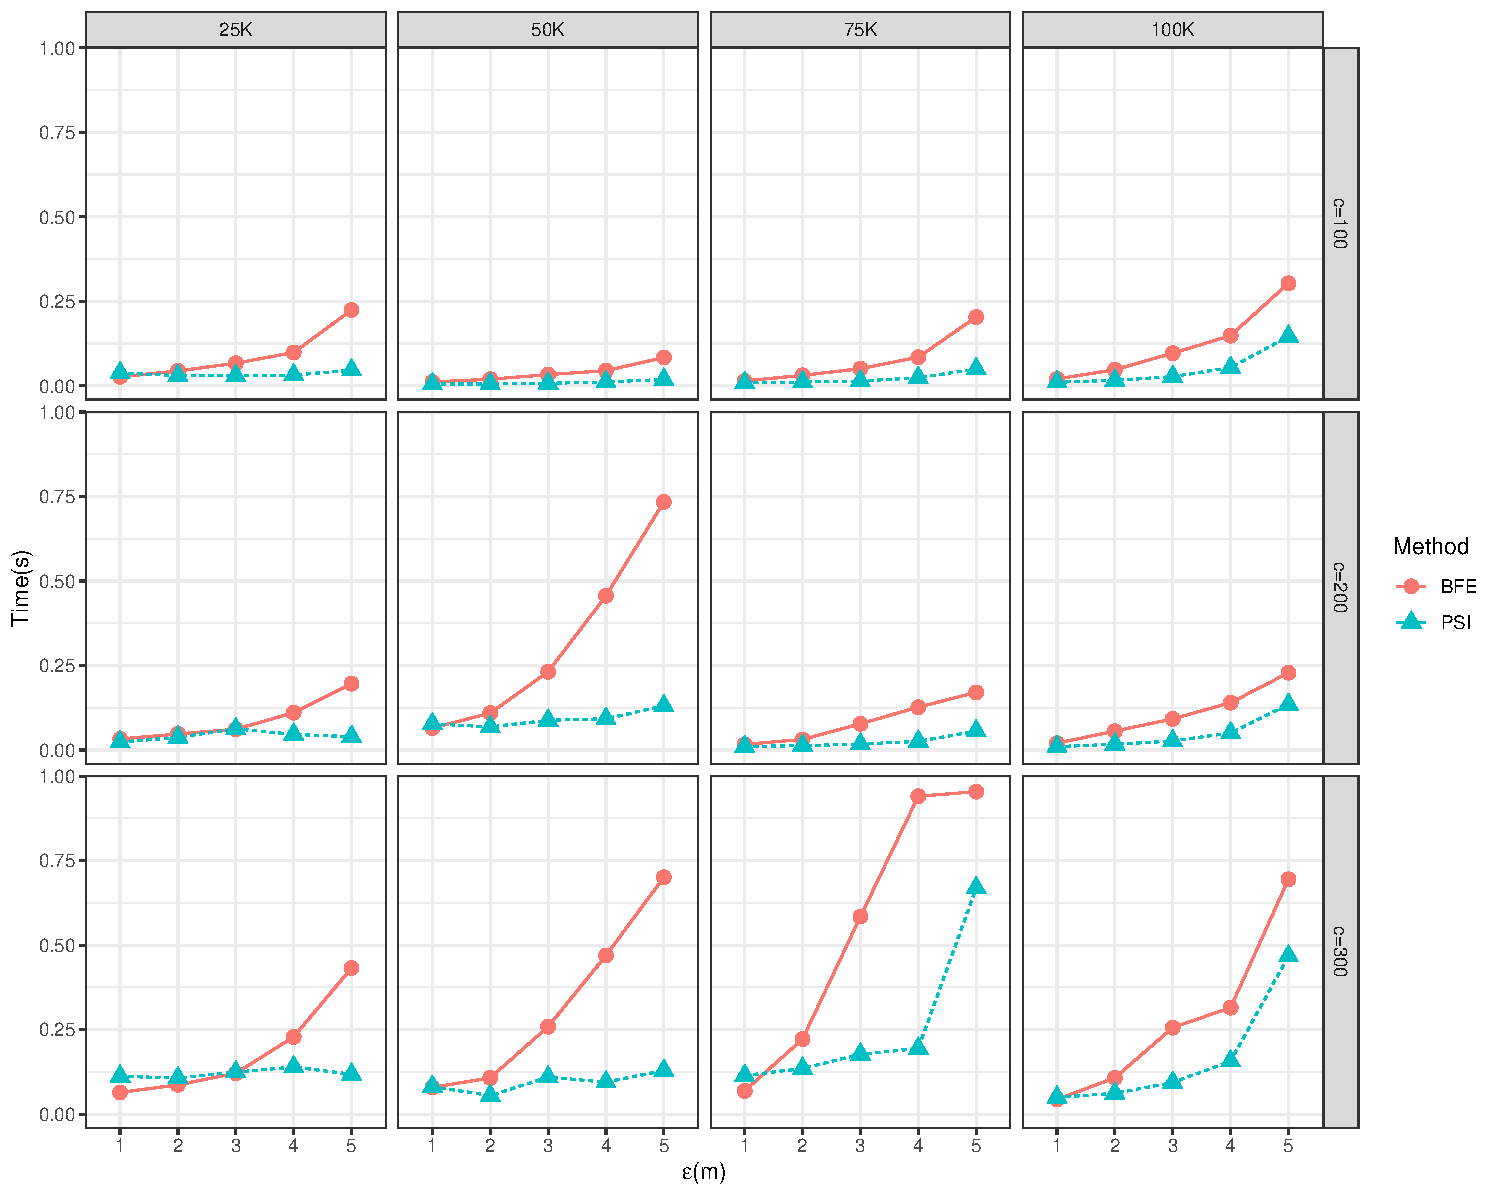
\includegraphics[width=\linewidth]{figures/plots/05_uniform_performance/uniform_performance.pdf}
    \caption{Performance in an uniform dataset analysing density and capacity with diverse values for epsilon.}\label{fig:uniform_performance}
\end{figure}

\subsection{Evaluation of Phase 2: Temporal join.}
Phase 2 deals with the joining of maximal disks between time instants to create the flocks. In Section \ref{sec:temporal_join} we discussed four alternatives: Master, Level, LCA and Cube-based. For these experiments we use the scalable PSI approach given its robust performance. First we compared the Master and By-Level alternatives for varying $\varepsilon$ from 20 to 40m using the Berlin10K dataset (see Figure \ref{fig:step_performance}). For By-Level we examined different options for the Step (from 1 to 6). The Master approach is the slowest given the overhead of sending all the CPFs to the root node. The By-Level approach performance depends on the Step. Small step (i.e. step 1) adds the overhead that CPFs may need to be evaluated in more intermediate nodes until completed. A larger Step value reduces parallelism as more CPFs are send to intermediate nodes. Based on these experiments we set Step=3.

We also evaluated the best value for the \textit{interval} parameter for the Cube-based approach. We tested different values for the interval parameter using the LA25K dataset with $\varepsilon=30m$. This dataset has a total of 30 time instants, and we varied the interval parameter from 2 to 12 time instants.  The results appear in Figure \ref{fig:interval_performance}. Lower interval values imply higher parallelism (more cubes that can be processed independently) but we need to check more cube crossings for CPFs which adds to the execution time. On the other hand, large intervals, reduce parallelism but also reduce the number of CPF crossings. Based on these results, we set $interval=6$ for the Cube-based approach.   

\begin{figure}
    \centering
    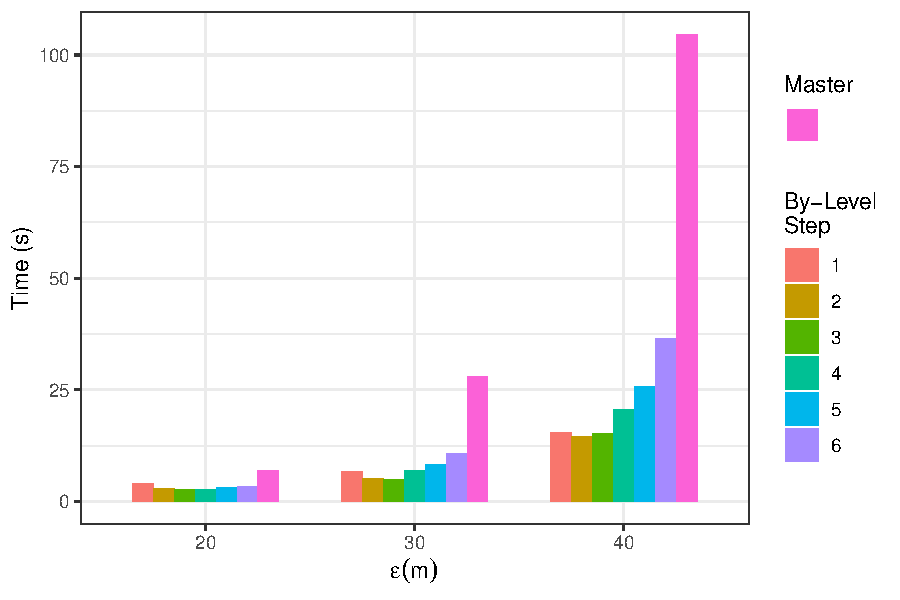
\includegraphics[width=0.8\linewidth]{figures/plots/06_step_performance/step_performance.pdf}
    \caption{Root and step alternative for temporal join using the Berlin dataset (step=7 is root).}\label{fig:step_performance}
\end{figure}

\begin{figure}
    \centering
    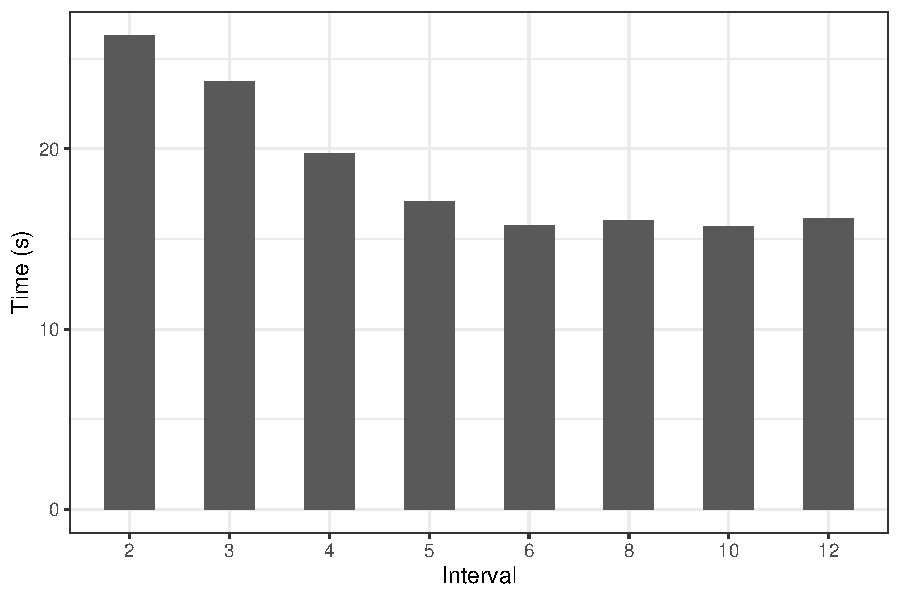
\includegraphics[width=0.8\linewidth]{figures/plots/07_interval_performance/interval-performance.pdf}
    \caption{Interval analysis for the Cube-based alternative for temporal join using the LA25K dataset.}\label{fig:interval_performance}
\end{figure}

Finally we compared the above optimized versions of By-Level and Cube-based with Master and LCA. Figure \ref{fig:la25k_e_bfe_psi} shows the results, including the sequential PSI algorithm for reference. This experiment used the LA25K dataset while varying the value of $\varepsilon$ from 5 to 30m. Clearly, all parallel approaches offer large improvement. To further analyse the relative performance of the scalable approaches, Figure \ref{fig:la25k_e} focuses on their performance for the same experiment. Interestingly, for very small $\varepsilon$ the Master approach is the best (simply because there are not many flocks, so sending the CPFs to one node is fast). As $\varepsilon$ increases, the Cube-based approach is the winner as it takes more advantage of parallelism. At the same scenario, By-Level improves over Master for the reasons explained in Figure \ref{fig:step_performance}). Similarly, for larger $\varepsilon$ LCA is faster than By-Level because it finds faster the node that can complete the CPFs.
We run the same experiment using the LA50K dataset while varying the value of $\varepsilon$ from 4 to 20m. The results appear in Figure \ref{fig:la50k_e}. Again, the Cube-based approach has the best performance as $\varepsilon$ increases.

\begin{figure}
    \centering
    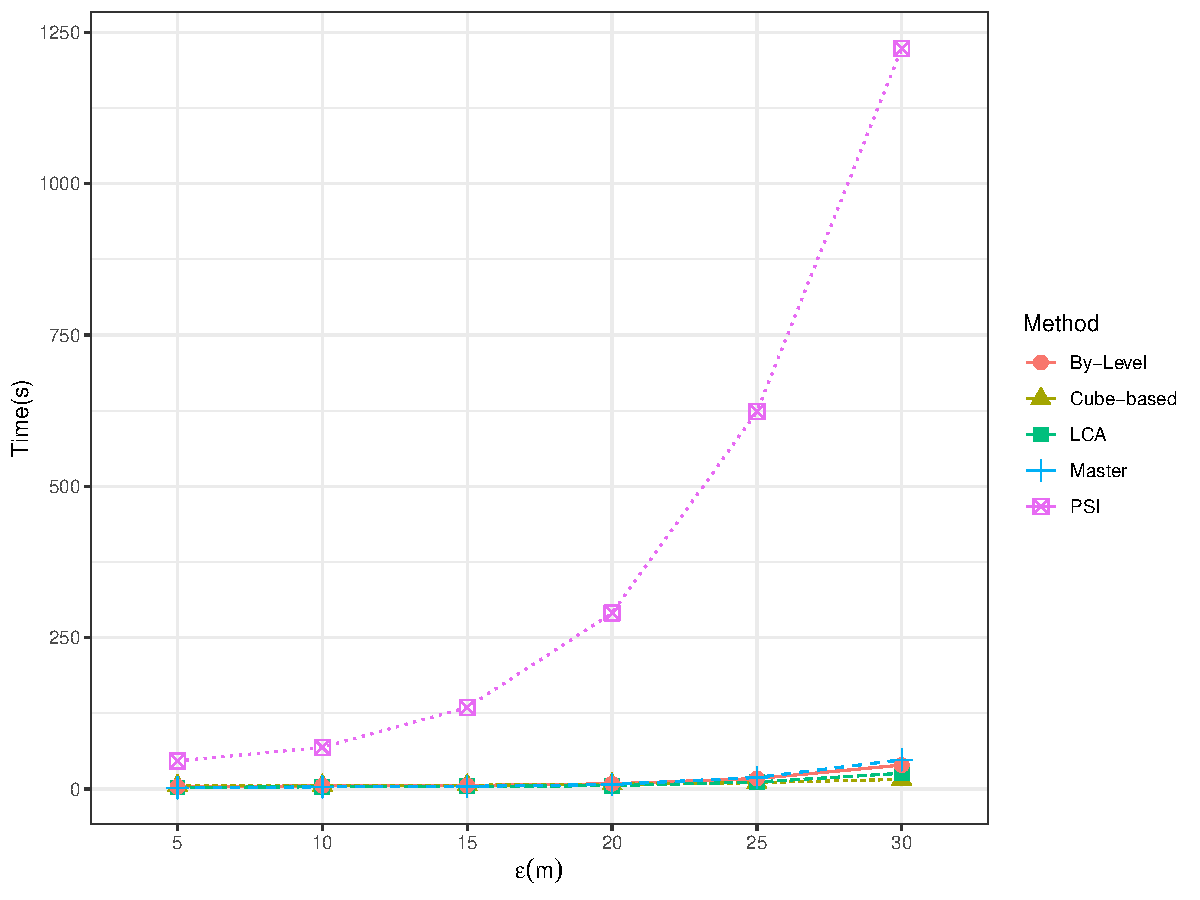
\includegraphics[width=0.75\linewidth]{figures/plots/08_sequential_parallel/la25k_e_bfe_psi.pdf}
    \caption{Performance comparing parallel and sequential alternatives in the LA25K dataset.}\label{fig:la25k_e_bfe_psi}
\end{figure}

\begin{figure}
    \centering
    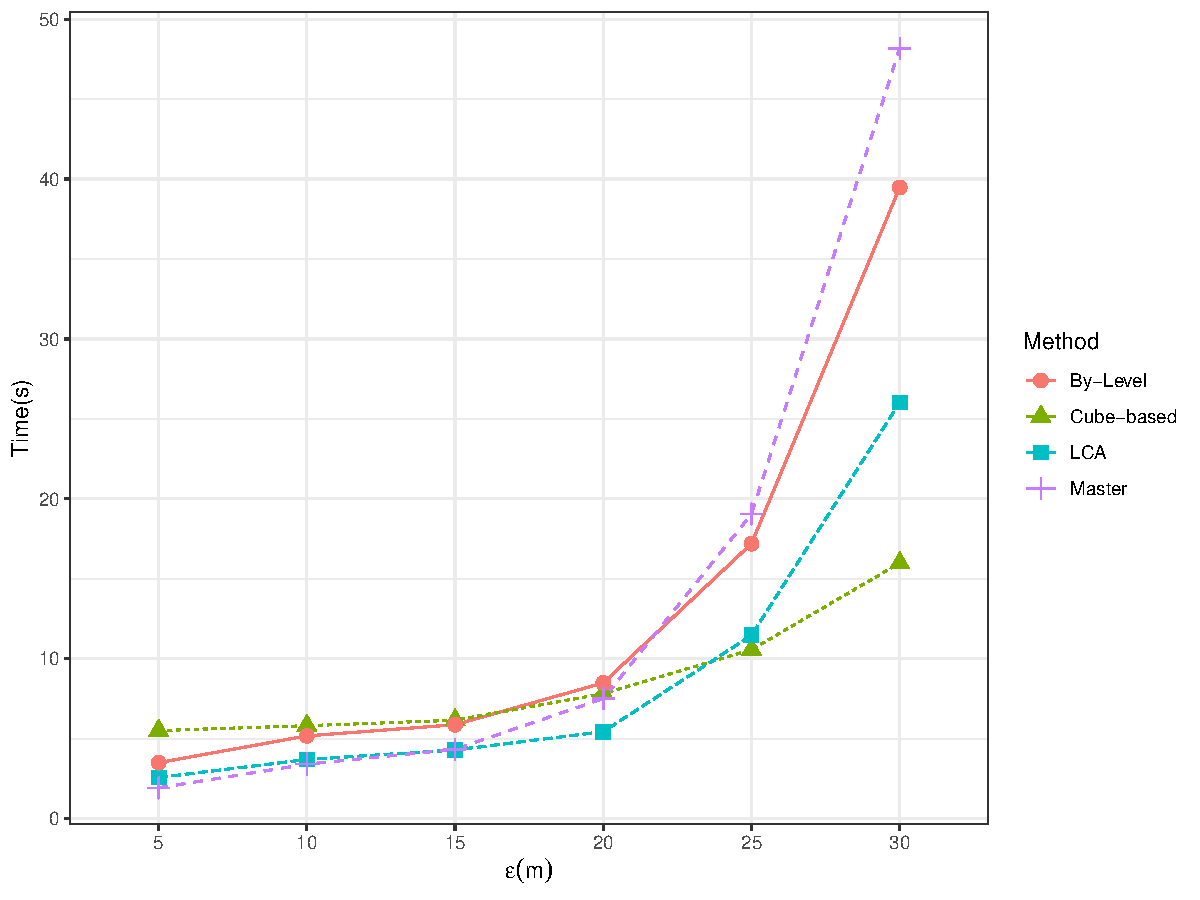
\includegraphics[width=0.75\linewidth]{chapter4/figures/plots/08_sequential_parallel/la25k_e}
    \caption{Performance of the 4 parallel alternatives in the LA25K dataset.}\label{fig:la25k_e}
\end{figure}

\begin{figure}
    \centering
    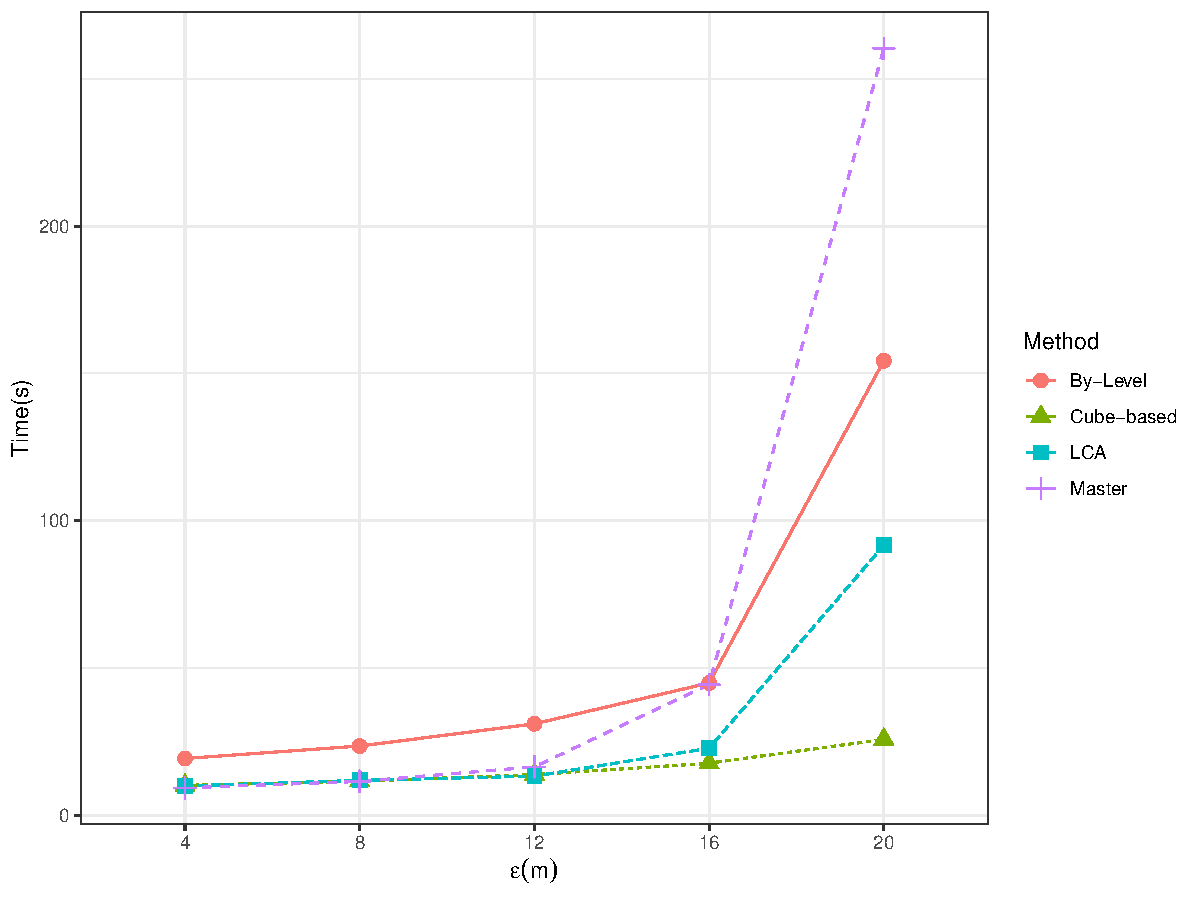
\includegraphics[width=0.75\linewidth]{chapter4/figures/plots/08_sequential_parallel/la50k_e}
    \caption{Performance of the 4 parallel alternatives in the LA50K dataset.}\label{fig:la50k_e}
\end{figure}
